%%%%%%%%%%%%%%%%%%%%%%%%%%%%%%%%%%%%%%%%%
% University/School Laboratory Report
% LaTeX Template
% Version 3.1 (25/3/14)
%
% This template has been downloaded from:
% http://www.LaTeXTemplates.com
%
% Original author:
% Linux and Unix Users Group at Virginia Tech Wiki 
% (https://vtluug.org/wiki/Example_LaTeX_chem_lab_report)
%
% License:
% CC BY-NC-SA 3.0 (http://creativecommons.org/licenses/by-nc-sa/3.0/)
%
%%%%%%%%%%%%%%%%%%%%%%%%%%%%%%%%%%%%%%%%%

%----------------------------------------------------------------------------------------
%	PACKAGES AND DOCUMENT CONFIGURATIONS
%----------------------------------------------------------------------------------------

\documentclass{article}

\usepackage[version=3]{mhchem} % Package for chemical equation typesetting
\usepackage{siunitx} % Provides the \SI{}{} and \si{} command for typesetting SI units
\usepackage{graphicx} % Required for the inclusion of images
\usepackage{natbib} % Required to change bibliography style to APA
\usepackage{amsmath} % Required for some math elements 
\usepackage{hyperref} % Add link to text
\usepackage{comment} % Enable comment blocks

\setlength\parindent{0pt} % Removes all indentation from paragraphs

\renewcommand{\labelenumi}{\alph{enumi}.} % Make numbering in the enumerate environment by letter rather than number (e.g. section 6)

%\usepackage{times} % Uncomment to use the Times New Roman font

%----------------------------------------------------------------------------------------
%	DOCUMENT INFORMATION
%----------------------------------------------------------------------------------------

\title{Modeling Modes of Operation \\ Using AADL and AGREE } % Title

\author{Danielle Stewart} % Author name

\date{April 2019} % Date for the report

\begin{document}

\maketitle % Insert the title, author and date

%\begin{center}
%\begin{tabular}{l r}
%Date Performed: & April, 2019 \\ % Date the experiment was performed
%Partners: & James Smith \\ % Partner names
%& Mary Smith \\
%Instructor: & Professor Heimdahl % Instructor/supervisor
%\end{tabular}
%\end{center}

% If you wish to include an abstract, uncomment the lines below
% \begin{abstract}
% Abstract text
% \end{abstract}

%----------------------------------------------------------------------------------------
%	SECTION 1
%----------------------------------------------------------------------------------------


%%%%%%%%%%%%%%%%%%%%%%%%%%%%%%%%%%%%%%%%%%%%%%%%%%%%
%				Problem Description
%%%%%%%%%%%%%%%%%%%%%%%%%%%%%%%%%%%%%%%%%%%%%%%%%%%%
\section{The Point of it All}

In critical system development, it's important to have redundancy in the system and introduce modes of operation. For instance when everything works properly, we are in normal mode. If a failure occurs in normal mode, we can switch to a backup or alternate mode, and so on. When modeling this in AADL and AGREE for a large scale Wheel Brake System, we ran into some issues once we generated minimal cut sets. For minimal cut sets of cardinality 1, faults were showing up in normal and alternate mode. This shouldn't be happening if the behavior of the components is modelled correctly. If a fault occurs in normal mode, the system should automatically switch to alternate mode and still provide the service as intended. For a system with $n$ backup modes (or redundancy plans), we should see tolerance up to $n$ faults.

First I will briefly describe the Wheel Brake System and then describe the small scale system created to sort out what contracts are needed to enforce switching modes and testing such behavior. For a more detailed description of the large scale WBS, see the Tech Report: \url{https://www.cs.umn.edu/sites/cs.umn.edu/files/tech_reports/18-007_0.pdf}.
 
The small scale system used to implement and test switching modes is located in repository: \url{https://github.com/dkstewart/University-Research/tree/master/Models} and is titled \textit{Modes of Operation}.

\subsection{WBS Problem Description}
The overall behavior of the WBS is simple enough. When the brakes are commanded, we should recieve brake force at the wheel. There are three operating modes in the WBS model. In \textit{normal} mode, the system uses the \textit{green} hydraulic circuit. In \textit{alternate} mode, the system uses the \textit{blue} hydraulic circuit. The last mode of operation is the \textit{emergency} mode. This mode is entered if the blue hydraulic line fails. The accumulator pump has a reserve of pressurized hydraulic fluid and will supply this to the blue circuit in emergency mode.

In Figure~\ref{fig:wbs}, the simplified architectural structure of the WBS can be seen. The blue, green, and accumulator pumps are shown and the main idea of the structure is shown. The \textit{selector} valve selects which line the system utilizes and the accumulator input occurs when no blue output is provided from the selector valve. 

\begin{figure}[h]
\begin{center}
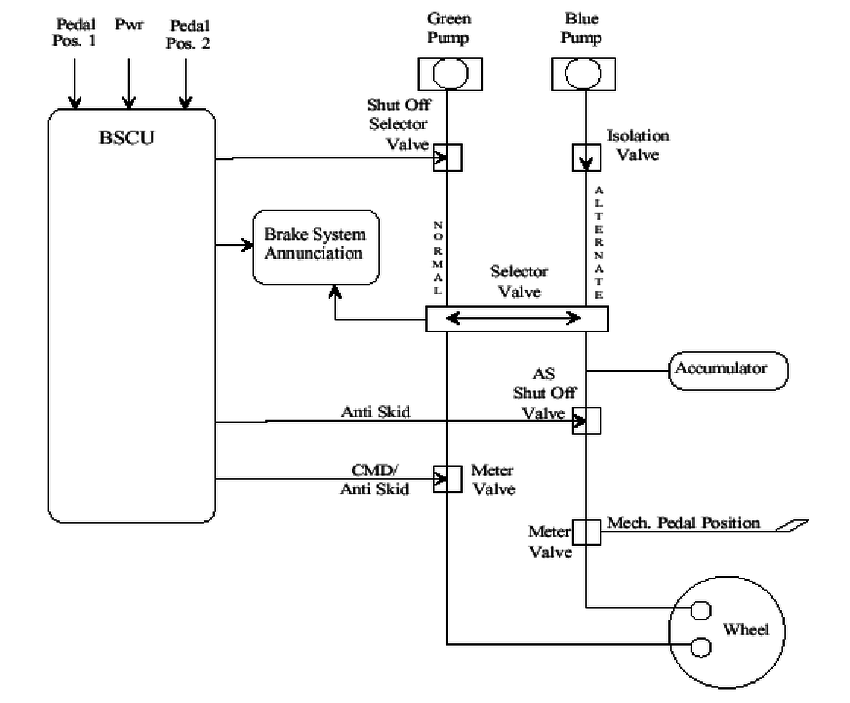
\includegraphics[width=0.65\textwidth]{images/wbs_arp4761} 
\caption{Simple Structure of the WBS System}
\label{fig:wbs}
\end{center}
\end{figure}

Once the system switches modes, it does not switch back. This point becomes important later when we talk about enforcing mode behavior through contracts.

What is not shown in the figure is the presence of a \textit{monitor system} in the WBS that monitors the health of the system and determines if the system is providing valid electrical commands. This component provides a \textit{sys\_valid} variable to signal if we have healthy commands coming from the \textit{braking system control unit}. 

When generating MinCutSets, single points of failure were located in the normal and alternate modes of operation. The point of multiple modes of operation is to \textit{avoid} single points of failure. Thus it was clear there was something wrong with the contracts of the model. Given the size of the WBS, it was prudent to put together a small scale model similar in nature to the WBS. This allows the easy addition of contracts and testing to make sure that we have desired behavior with regard to these modes. 

%%%%%%%%%%%%%%%%%%%%%%%%%%%%%%%%%%%%%%%%%%%%%%%%%%%%
%				Modes of Operation Description
%%%%%%%%%%%%%%%%%%%%%%%%%%%%%%%%%%%%%%%%%%%%%%%%%%%%
\section{Modes of Operation Model Description}
The smaller model was built based off of the general architectural structure (subcomponents and connections) of the WBS. 
\begin{figure}[h]
\begin{center}
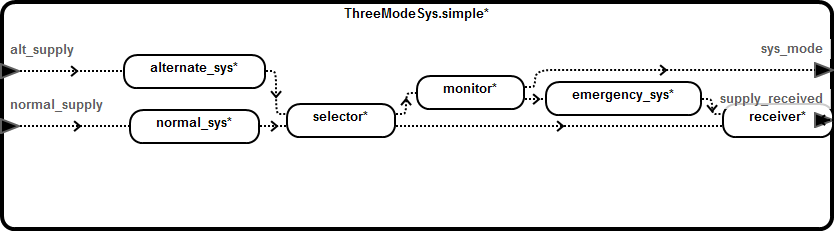
\includegraphics[width=0.95\textwidth]{images/modes_flows} 
\caption{Information Flows of the Modes of Operation System}
\label{fig:modes1}
\end{center}
\end{figure}
Top level has supply as inputs. This "supply" is always positive and never zero. 

Subcomponents: 
\begin{itemize}
\item Normal : Takes supply input from top level. Contract guarantees that supply out equals supply in. Output sent to Selector. Fault defined for this subcomponent is: stuck at zero output.
\item Alternate : Takes supply input from top level. Contract guarantees that supply out equals supply in. Output sent to Selector. Fault defined for this subcomponent is: stuck at zero output.

\item Selector : is a valve that takes the supply from both normal and alternate components and selects between them. Its behavior is very much like the selector valve in the WBS. The behavior is a bit more involved for this component. 

Inputs: normal\_supply, alt\_supply \\
Outputs: valve\_position, supply\_out\\

The valve position indicates which supply the system is currently using. It is defined as follows. \\
Position 1: Normal supply\\
Position 2: Alternate supply\\
Position 3: Neither (emergency signal)\\

\underline{Normal supply behavior}: 

Normal is supplied and we were previously in normal mode \\
$(normal\_supply > 0) \land (prev(valve\_position) = 1)$ 

Valve position is 1.

\underline{Alternate supply behavior}: 

Case 1: Previously normal mode, normal supplies nothing, alternate is supplied \\
$(((normal\_supply \leq 0) \land (alt\_supply > 0) \land prev(valve\_position) = 1)$ 

Case 2: Previously alternate mode, alternate is supplied \\
$((alt\_supply > 0) \land prev(valve\_position) = 2))$

In both cases, valve position is 2.

\underline{Emergency supply behavior}: 

Case 1: Previously normal, neither normal nor alternate are supplied \\
$prev(valve\_position) = 1) \land (alt\_supply \leq 0) \land (normal\_supply \leq 0)$

Case 2: Previously alternate, alternate supplies zero \\
$prev(valve\_position) = 2 \land (alt\_supply \leq 0)$

Case 3: Previously emergency \\
$prev(valve\_position) = 3$

In all three cases, we set valve\_position to 3. 

This logic also ensures that we do not switch back to previous modes. This is clearly seen by the use of the \textit{prev} statements. When previously in a certain mode, we keep it that way (or move on to a more serious mode). If it is desired to let the system switch back to previous modes, this is the component that would regulate that logic for the most part.

The \underline{supply output} guarantee links the valve position with which input we use to equate with the output. 

if ($valve\_position = 1$) then ($normal\_supply = supply\_out$)\\
else if ($valve\_position = 2$) then ($alt\_supply = supply\_out$)\\
else ($supply\_out = 0$)\\

\item Monitor : Monitors the mode of the system (similar to the MonitorSystem in WBS). It gets input from the Selector on whether its getting supply from normal or alternate and if the supply is not received at Selector, then it sends command to Emergency. Emergency then sends pressure to Receiver. The system mode is sent to the top level for testing purposes.

The logic of the monitor is surprisingly simple. The selector sends valve postion and based on the valve position, the system mode is determined. When the valve is in position 3 (indicating selector is getting no supply from  normal or alternate), the monitor sends emergency command to emergency subcomponent. The system mode is then sent to the top level for testing purposes. 

\item Emergency : Backup reserve supply. If there is a command from the monitor to activate emergency system, then supply output is a constant value (5). Else output is zero. Fault defined for this subcomponent is: stuck at zero output. 

\item Receiver : the "end of the flow" subcomponent that needs to receive the supply. Similar to the wheel in WBS. It takes input from the selector and from the emergency component. The only output is to the top level stating that it has (or has not) received supply. 

\end{itemize}

The logic is very basic. If no normal supply at selector, then switch to alternate. Likewise alternate switch to emergency. Faulty behavior is defined when the supply is zero. The bulk of the necessary logic in order to make these mode changes resides in the selector. The cases that cover what mode system is in was important to get right and took some trial and error (i.e. studying counterexamples that showed the missing cases).

\begin{figure}[h]
\begin{center}
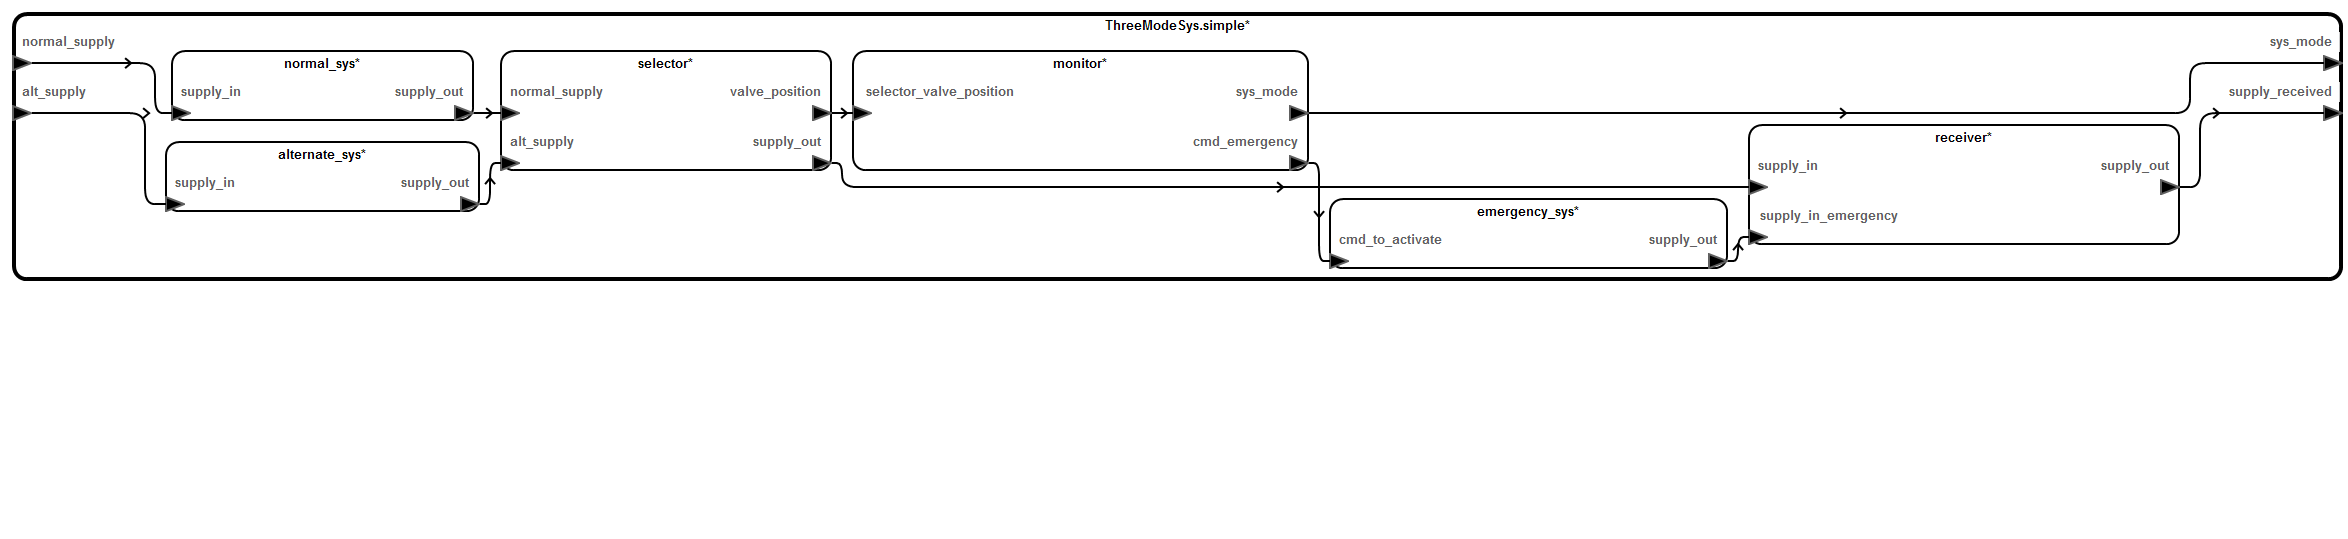
\includegraphics[width=1.2\textwidth]{images/modes_structure} 
\caption{Architecture of the Modes of Operation System}
\label{fig:modes2}
\end{center}
\end{figure}

\section{Top Level Contracts}
The main contracts of interest are shown in Figure~\ref{fig:lemmas}. In particular, the first lemma \textit{``Receiver supply is always positive''} can indicate single points of failure when faults are activated. Given either 1 or 2 active faults in the system, this lemma still proves. This is sufficient to show that the system does in fact switch modes. 

\begin{figure}[h]
\begin{center}
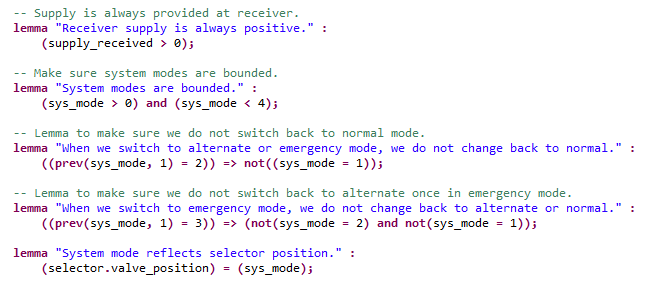
\includegraphics[width=1.2\textwidth]{images/lemmas} 
\caption{Top Level Contracts}
\label{fig:lemmas}
\end{center}
\end{figure}

There are no MinCutSets of cardinality one for this system. The simple fault tree is shown in Figure~\ref{fig:ft}.

\begin{figure}[h]
\begin{center}
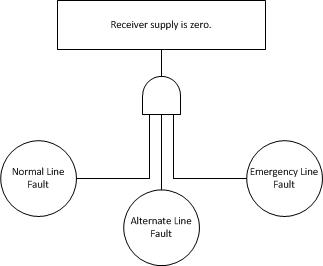
\includegraphics[width=0.45\textwidth]{images/ft} 
\caption{Fault Tree}
\label{fig:ft}
\end{center}
\end{figure}


\section{Difficulties, Thoughts, Tips}
The biggest key was the behavior of the selector valve. Every counterexample displayed a missing case and that was incredibly helpful to make sure all cases were covered. Once that was in place, the job was finished. Since the smaller model was based on the WBS, the behavior/contracts of the selector valve and monitor will have to be studied to make sure they are compatible with the smaller model. Easier said than done, right? :)


















% If you have more than one objective, uncomment the below:
%\begin{description}
%\item[First Objective] \hfill \\
%Objective 1 text
%\item[Second Objective] \hfill \\
%Objective 2 text
%\end{description}

%\subsection{Definitions}
%\label{definitions}
%\begin{description}
%\item[Stoichiometry]
%The relationship between the relative quantities of substances taking part in a reaction or forming a compound, typically a ratio of whole integers.
%\item[Atomic mass]
%The mass of an atom of a chemical element expressed in atomic mass units. It is approximately equivalent to the number of protons and neutrons in the atom (the mass number) or to the average number allowing for the relative abundances of different isotopes. 
%\end{description} 
 
 \begin{comment}
 
%----------------------------------------------------------------------------------------
%	SECTION 2
%----------------------------------------------------------------------------------------

\section{Experimental Data}

\begin{tabular}{ll}
Mass of empty crucible & \SI{7.28}{\gram}\\
Mass of crucible and magnesium before heating & \SI{8.59}{\gram}\\
Mass of crucible and magnesium oxide after heating & \SI{9.46}{\gram}\\
Balance used & \#4\\
Magnesium from sample bottle & \#1
\end{tabular}

%----------------------------------------------------------------------------------------
%	SECTION 3
%----------------------------------------------------------------------------------------

\section{Sample Calculation}

\begin{tabular}{ll}
Mass of magnesium metal & = \SI{8.59}{\gram} - \SI{7.28}{\gram}\\
& = \SI{1.31}{\gram}\\
Mass of magnesium oxide & = \SI{9.46}{\gram} - \SI{7.28}{\gram}\\
& = \SI{2.18}{\gram}\\
Mass of oxygen & = \SI{2.18}{\gram} - \SI{1.31}{\gram}\\
& = \SI{0.87}{\gram}
\end{tabular}

Because of this reaction, the required ratio is the atomic weight of magnesium: \SI{16.00}{\gram} of oxygen as experimental mass of Mg: experimental mass of oxygen or $\frac{x}{1.31}=\frac{16}{0.87}$ from which, $M_{\ce{Mg}} = 16.00 \times \frac{1.31}{0.87} = 24.1 = \SI{24}{\gram\per\mole}$ (to two significant figures).

%----------------------------------------------------------------------------------------
%	SECTION 4
%----------------------------------------------------------------------------------------

\section{Results and Conclusions}

The atomic weight of magnesium is concluded to be \SI{24}{\gram\per\mol}, as determined by the stoichiometry of its chemical combination with oxygen. This result is in agreement with the accepted value.

%\begin{figure}[h]
%\begin{center}
%
\includegraphics[width=0.65\textwidth]{placeholder} % Include the image placeholder.png
%\caption{Figure caption.}
%\end{center}
%\end{figure}

%----------------------------------------------------------------------------------------
%	SECTION 5
%----------------------------------------------------------------------------------------

\section{Discussion of Experimental Uncertainty}

The accepted value (periodic table) is \SI{24.3}{\gram\per\mole} \cite{Smith:2012qr}. The percentage discrepancy between the accepted value and the result obtained here is 1.3\%. Because only a single measurement was made, it is not possible to calculate an estimated standard deviation.

The most obvious source of experimental uncertainty is the limited precision of the balance. Other potential sources of experimental uncertainty are: the reaction might not be complete; if not enough time was allowed for total oxidation, less than complete oxidation of the magnesium might have, in part, reacted with nitrogen in the air (incorrect reaction); the magnesium oxide might have absorbed water from the air, and thus weigh ``too much." Because the result obtained is close to the accepted value it is possible that some of these experimental uncertainties have fortuitously cancelled one another.

%----------------------------------------------------------------------------------------
%	SECTION 6
%----------------------------------------------------------------------------------------

\section{Answers to Definitions}

\begin{enumerate}
\begin{item}
The \emph{atomic weight of an element} is the relative weight of one of its atoms compared to C-12 with a weight of 12.0000000$\ldots$, hydrogen with a weight of 1.008, to oxygen with a weight of 16.00. Atomic weight is also the average weight of all the atoms of that element as they occur in nature.
\end{item}
\begin{item}
The \emph{units of atomic weight} are two-fold, with an identical numerical value. They are g/mole of atoms (or just g/mol) or amu/atom.
\end{item}
\begin{item}
\emph{Percentage discrepancy} between an accepted (literature) value and an experimental value is
\begin{equation*}
\frac{\mathrm{experimental\;result} - \mathrm{accepted\;result}}{\mathrm{accepted\;result}}
\end{equation*}
\end{item}
\end{enumerate}

%----------------------------------------------------------------------------------------
%	BIBLIOGRAPHY
%----------------------------------------------------------------------------------------

\bibliographystyle{apalike}

\bibliography{biblio}

%----------------------------------------------------------------------------------------
\end{comment}

\end{document}